\ExerciseAppendix

\begin{enumerate}
\def\labelenumi{\arabic{enumi})}
\tightlist
\item
  设 X 是其上定义了一个以乘法记号书写的结合合成律的豪斯多夫拓扑空间。把定义 1 推广到 X 的元素的族 \((x_{i})_{i\in I}\)（其指标集 I 线性有序）的情形。对 I 的每个有限子集 J，令 \(p_{J}\) 表示乘积 \(\prod_{i\in J} x_{i}\)，即序列 \((x_{i})_{i\in J}\) 的乘积。
\end{enumerate}

若 X 是完备拓扑群，则 X 的点的族 \((x_{i})_{i\in\mathbf{I}}\) 是可乘的，当且仅当：对 X 的单位元 e 的任一邻域 V，存在 I 的有限子集 \(J_{0}\)，使对包含 \(J_{0}\) 的 I 的每个有限子集 J，有 \(p_{J}(p_{J_{0}})^{-1}\in V\){[}或 \((p_{J_{0}})^{-1}p_{J}\in V\){]}。

\begin{enumerate}
\def\labelenumi{\arabic{enumi})}
\setcounter{enumi}{1}
\tightlist
\item
  在线性有序集 I 中，我们称非空子集 J 为 I 的一个截段，如果每当 \(\alpha\) 与 \(\beta\) 是 J 的使 \(\alpha < \beta\) 的元素时，有 \([\alpha, \beta] \subset J\)。
\end{enumerate}

\begin{enumerate}
\def\labelenumi{\alph{enumi})}
\item
  设 \((x_{i})_{i\in J}\) 是完备群 G 中的可乘族。试证：对每个截段 \(J\)（\(I\) 的），族 \((x_{i})_{i\in J}\) 是可乘的（先考虑特殊情形：\(J\) 的不属于 \(J\) 的下界组成的集为空）。
\item
  分划 \((\mathrm{J}_{\lambda})_{\lambda \in \mathbf{L}}\)（\(\mathbf{I}\) 的）称为有序分划，如果 \(\mathbf{L}\) 是线性有序集，且关系 \(\lambda < \mu, \alpha \in \mathrm{J}_{\lambda}, \beta \in \mathrm{J}_{\mu}\) 蕴含 \(\alpha < \beta\)；诸 \(\mathrm{J}_{\lambda}\) 于是都是 \(\mathbf{I}\) 的截段。若 \((x_{t})_{t \in \mathbf{I}}\) 是完备群 \(\mathbf{G}\) 中的可乘族，试证：若令 \(p_{\lambda} = \prod_{t \in J_{\lambda}} x_{t}\)，则族 \((\mathrm{P}_{\lambda})_{\lambda \in \mathbf{L}}\) 是可乘的，且与族 \((x_{t})_{t \in \mathbf{I}}\) 有相同的积。c) 反之，若 \((\mathrm{J}_{\lambda})_{\lambda \in \mathbf{L}}\) 是 \(\mathbf{I}\) 的有限有序分划，且 \((x_{t})_{t \in \mathbf{I}}\) 使诸族 \((x_{t})_{t \in J_{\lambda}}\) 中的每一个都是可乘的，则族 \((x_{t})_{t \in \mathbf{I}}\) 是可乘的。
\end{enumerate}

\begin{enumerate}
\def\labelenumi{\arabic{enumi})}
\setcounter{enumi}{2}
\tightlist
\item
  设 G 是豪斯多夫拓扑群，它具有单位元 e 的一个邻域 \(V_{0}\)，\(x \to x^{-1}\) 在其上一致连续（作为映射 \(G_{d} \to G_{d}\)：参见第 III 章，§ 3，习题 7 与 8）。设 \((x_{i})_{i\in I}\) 是 G 的点的可乘族；试证：对 e 的每个邻域 U，存在 I 的有限子集 \(J_{0}\)，使对含于 I 的不与 \(J_{0}\) 相交的某截段中的 I 的每个有限子集 K，有 \(p_{k}\in U\)。{[}先证明存在 I 的有限子集 \(H_{0}\) 与 G 的有限个点 \(a_{1},a_{2},\ldots,a_{q}\)，使对含于 I 的不与 \(H_{0}\) 相交的某截段中的 I 的每个有限子集 L，有 \(p_{L}\in a_{k}V_{0}^{\prime}a_{k}^{-1}\)（对至少一个指标 k），其中 \(V_{0}^{\prime}\) 是 e 的使 \(V_{0}^{\prime}V_{0}^{\prime}\subset V_{0}\) 的邻域。于是我们可限于考虑含于以 \(H_{0}\) 的两个相继指标为端点的开区间之一的有限子集；利用习题 2 a) 的论证以及 \(x^{-1}\) 在每个邻域 \(a_{k}V_{0}a_{k}^{-1}\) 上的一致连续性。{]}
\end{enumerate}

由此推出：在同一条件下，关于 I 的有限子集的余集的滤子（若 I 无限），有 \(\lim x_{t}=e\)。

\begin{enumerate}
\def\labelenumi{\arabic{enumi})}
\setcounter{enumi}{3}
\item
  设 G 是局部紧群。若 \((x_{t})\) 是 G 的点的可乘族，试证该族的有限部分积 \(p_{J}\) 组成的集是相对紧的。
\item
  \begin{enumerate}
  \def\labelenumii{\alph{enumii})}
  \tightlist
  \item
    设 G 是完备群，G 中单位元 e 的每个邻域都包含 G 的开子群。试证：G 的点的序列 \((x_{n})\) 是可乘的，当且仅当 \(\lim_{n\to\infty}x_{n}=e\)。
  \end{enumerate}
\end{enumerate}

\begin{enumerate}
\def\labelenumi{\alph{enumi})}
\setcounter{enumi}{1}
\tightlist
\item
  设 G 是完备群，其中 e 的每个邻域都包含 G 的正规开子群。试证：G 的点的族 \((x_{t})_{t\in I}\) 是可乘的，当且仅当关于 I 的有限子集的余集的滤子有 \(\lim x_{t}=e\)（利用习题 3）。
\end{enumerate}

\begin{enumerate}
\def\labelenumi{\arabic{enumi})}
\setcounter{enumi}{5}
\tightlist
\item
  设 \(\mathbf{A}\) 是（\(\mathbf{R}\) 上的）由定义在区间 \(\mathbf{X} = [1, +\infty[\)（\(\mathbf{R}\) 中的）上的有界实值函数组成的代数，赋以范数 \(||f|| = \sup_{x\in \mathbf{X}}|f(x)|\)。
\end{enumerate}

对每个整数 \(n > 0\)，令 \(u_{n}\) 是这样的函数：它等于 \(\mathbf{1} / n\)（当 \(n \leqslant x \leqslant n + 1\)），而在别处等于 \(0\)。试证：族 \((1 + u_n)\) 在 \(\mathbf{A}\) 中是可乘的，但以 \(u_{n}\) 为通项的级数在 \(\mathbf{A}\) 中不是绝对可和的。

\begin{enumerate}
\def\labelenumi{\arabic{enumi})}
\setcounter{enumi}{6}
\item
  设 \((\pmb{x}_n)\) 是赋范代数 \(\mathbf{A}\) 的点的序列，使得对每个置换 \(\sigma\)（\(\mathbf{N}\) 的），以 \(x_{\sigma(n)}\) 为通项的无穷乘积收敛且 \(\mathbf{P}_{n=0} x_{\sigma(n)}\) 是单位。试证：每个序列 \((x_{\sigma(n)})\) 都是可乘的（论证与第 III 章，§ 5，第 7 号命题 9 相同）。
\item
  设 A 是完备赋范代数。试证：若 \((x_{n})\) 是 A 的点的序列，使得对每个置换 \(\sigma\)（N 的），序列 \((x_{\sigma(n)})\) 是可乘的且其积是单位，则每个 \(x_{n}\) 都是单位。（先建立下面的代数引理：在带单位元素的环中，若两个元素 x, y 使 xy 是单位而 yx 不是零因子，则 x 与 y 都是单位。）
\end{enumerate}

\begin{center}\textbf{拓扑空间的主要类型图解}\end{center}

\pandocbounded{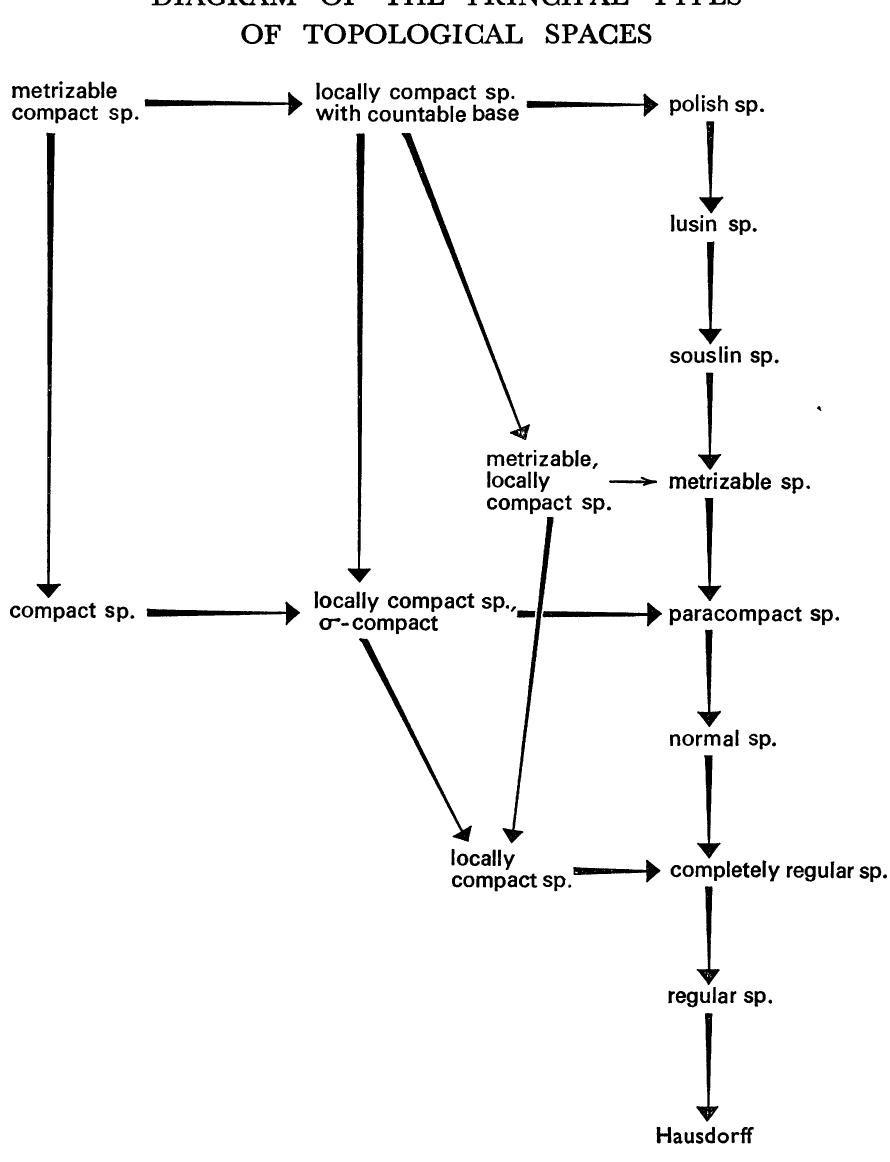
\includegraphics[keepaspectratio]{images/part002_2eb706e7.jpg}}

